% ============================================================
% FINAL PROJECT REPORT - ENGLISH VERSION
% Project 15: Document-Image Machine Translation (imgtrans)
% Course: CSC15012 - Applications of NLP in Industry
% Student: Le Dinh Minh Quan - 23127460 - 23CNTThuc
% ============================================================
\documentclass[12pt,a4paper]{article}

\usepackage[utf8]{inputenc}
\usepackage{geometry}
\geometry{left=2.3cm, right=2.3cm, top=2.5cm, bottom=2.5cm}
\usepackage{setspace}
\setstretch{1.25}
\usepackage{graphicx}
\usepackage{float}
\usepackage{booktabs}
\usepackage{longtable}
\usepackage{tabularx}
\usepackage{array}
\usepackage{hyperref}
\hypersetup{colorlinks=true, linkcolor=blue, urlcolor=blue, citecolor=blue, breaklinks=true}
\usepackage{xurl}
\usepackage{seqsplit}
\usepackage{listings}
\usepackage{xcolor}
\usepackage{amsmath}
\usepackage{caption}
\usepackage{subcaption}
\usepackage{enumitem}
\usepackage{fancyhdr}
\usepackage{tikz}
\usetikzlibrary{shapes.geometric, arrows.meta, positioning, fit, backgrounds, shadows}

% --- Make long inline code / paths break gracefully ---
\sloppy
\tolerance=2000
\emergencystretch=3em
\hbadness=10000
\setlength{\parskip}{0.15em}

% Helper for breakable monospaced paths
\newcommand{\bpath}[1]{\seqsplit{#1}}
\newcommand{\btt}[1]{\texttt{\seqsplit{#1}}}

% New column type for tabularx: left-aligned and ragged-right with breaking
\newcolumntype{L}{>{\raggedright\arraybackslash}X}

\lstset{
  basicstyle=\ttfamily\small,
  breaklines=true,
  frame=single,
  backgroundcolor=\color{gray!10},
  keywordstyle=\color{blue},
  commentstyle=\color{green!60!black},
  stringstyle=\color{red!70!black},
  showstringspaces=false,
  tabsize=2
}

\pagestyle{fancy}
\fancyhf{}
\fancyhead[L]{\small CSC15012 -- Final Project Report}
\fancyhead[R]{\small Le Dinh Minh Quan -- 23127460}
\fancyfoot[C]{\thepage}

% ============================================================
\begin{document}

% --- TITLE PAGE ---
\begin{titlepage}
\centering
\vspace*{0.5cm}

% HCMUS LOGO: upload logo_hcmus.png to Overleaf and uncomment the next line
\IfFileExists{logo_hcmus.png}{\includegraphics[width=3.5cm]{logo_hcmus.png}\\[0.5cm]}{}

{\large \textbf{VIETNAM NATIONAL UNIVERSITY HO CHI MINH CITY}}\\[0.3cm]
{\Large \textbf{UNIVERSITY OF SCIENCE}}\\[0.3cm]
{\large Faculty of Information Technology}\\[1.5cm]

{\LARGE \textbf{FINAL PROJECT REPORT}}\\[0.5cm]
{\large Course: \textbf{CSC15012 -- Applications of Natural Language\\ Processing in Industry}}\\[1.5cm]

{\Large \textbf{Project 15:}}\\[0.3cm]
{\Large \textbf{Document Image Machine Translation}}\\[0.3cm]
{\large A layout-preserving OCR $\rightarrow$ MT $\rightarrow$ render cascade with a deterministic agent}\\[2cm]

\begin{tabular}{ll}
\textbf{Student:} & Le Dinh Minh Quan \\
\textbf{Student ID:} & 23127460 \\
\textbf{Class:} & 23CNTThuc \\
\end{tabular}

\vfill
{\large Ho Chi Minh City, 2026}
\end{titlepage}

\tableofcontents
\newpage

% ============================================================
\section{Introduction}
% ============================================================

\textbf{In-image machine translation} -- the ``Google Translate camera'' experience -- takes an image, scan, or PDF that \emph{contains} text and produces a \emph{new image} in which the text has been translated into another language \emph{while preserving the original layout}. It is fundamentally different from plain document translation (text in $\rightarrow$ text out): the input and output are pixels, and the translated text must be drawn back exactly where the source text sat.

This project implements \texttt{imgtrans}, a complete, production-grade, license-clean pipeline for this task. The system is a \textbf{cascade}, not an end-to-end model:

\begin{itemize}
  \item an \textbf{OCR} front-end (Tesseract) reads the source text plus block boxes and per-word confidence;
  \item a \textbf{trainable machine-translation core} (\texttt{facebook/m2m100\_418M}, fine-tuned) translates each block -- the \emph{only} trained component;
  \item a \textbf{layout-preserving overlay renderer} (pure Pillow) erases each source box and re-draws the fitted, wrapped translation in place;
  \item a deterministic \textbf{agent (D1--D5)} orchestrates the cascade, gating on OCR confidence, translation quality, and overlay fit, and degrades gracefully (\texttt{overlay} $\rightarrow$ \texttt{side\_by\_side} $\rightarrow$ \texttt{needs\_review}) instead of producing a broken image.
\end{itemize}

OCR and rendering are pretrained or algorithmic; only the MT core is trained, with the Hugging Face \texttt{Seq2SeqTrainer} stack. The default direction is en$\rightarrow$fr, but because m2m100 is many-to-many ($\sim$100 languages), a single fine-tuned checkpoint also serves the multilingual requirement.

\textbf{Project Resources (public):}
\begin{itemize}\setlength\itemsep{0.15em}
  \item \textbf{GitHub repository (source code, MIT):} \url{https://github.com/ledinhminhquan/15_Document_Image_Translation}
  \item \textbf{Deployable surface:} FastAPI REST API + Gradio demo UI (mounted at \texttt{/ui}), a Docker image (Tesseract + Noto/DejaVu fonts + libGL baked in), and a one-button Colab H100 autopilot notebook. The system is \emph{deployable} but is \emph{not} currently hosted at a live public URL -- the deliverable is the API/UI/Docker/Colab capability described in Section~\ref{sec:deployment}.
\end{itemize}

% ============================================================
\section{Business Problem Definition}
% ============================================================

\subsection{Context and Motivation}

In-image translation is one of the most-used ``AI in the wild'' features (phone camera translate, manga scanlation, document-localization pipelines), yet it is rarely treated as an end-to-end engineering problem with honest metrics. The user always wants \emph{the page back}, translated -- not a disembodied list of strings. That ``render it back where it was'' requirement is the heart of the problem. Concrete settings:

\begin{itemize}
  \item \textbf{Travel signage, menus, and product labels} -- short, high-contrast text on cluttered/colored backgrounds, often rotated (the canonical ``point your camera'' case).
  \item \textbf{Scanned contracts and legal documents} -- layout (clauses, headers, signature blocks) carries meaning, so the translation must stay \emph{in place}.
  \item \textbf{Forms and official paperwork} -- field labels must be translated next to the right field, which only works if layout is preserved.
  \item \textbf{Screenshots and UI captures} -- text ``trapped'' in pixels with no selectable text layer.
  \item \textbf{Born-digital PDFs} -- already carry a text layer, so OCR can be \emph{bypassed} entirely (decision D2), giving zero OCR error.
\end{itemize}

\subsection{Target Users and Stakeholders}

\begin{itemize}
  \item \textbf{Newcomers, migrants, and travelers}: read a letter, form, sign, or notice in an unfamiliar language without a human translator at hand.
  \item \textbf{Document-localization teams}: a first-pass, layout-aware draft a human then reviews and corrects.
  \item \textbf{Developers}: an easy-to-integrate REST API and a containerized demo.
  \item \textbf{Trust \& safety / compliance}: the human-review (\texttt{needs\_review}) path keeps high-stakes documents under qualified human control.
\end{itemize}

\subsection{Problem Statement}

Given a page image, scan, or PDF, the system must:
\begin{enumerate}
  \item \textbf{Read} the source text plus block boxes and per-word confidence (OCR), or bypass OCR losslessly for born-digital PDFs;
  \item \textbf{Translate} each block (MT core), catching hallucination/truncation without a reference translation;
  \item \textbf{Render} the translation back into the original layout (overlay), or degrade to a side-by-side panel / honest \texttt{needs\_review} when an in-place overlay is infeasible.
\end{enumerate}

\subsection{Why NLP is Required}

The core difficulty is translation under uncertainty: OCR text is noisy and the target language is expressed with morphology, gender, register, and word-order that brittle dictionary or rule-based substitution cannot capture. A neural seq2seq MT model is required to translate coherent blocks faithfully, and reference-free verification (round-trip back-translation) is required to gate its output -- both are NLP problems with no rule-based shortcut.

\subsection{Success Metrics}

\begin{table}[H]
\centering
\caption{System success metrics across the four metric families}
\begin{tabular}{lll}
\toprule
\textbf{Type} & \textbf{Metric} & \textbf{Target / role} \\
\midrule
Business & Layout preserved (overlay usable) & Translation anchored to original structure \\
Business & Honest degradation (no silent garbage) & Flag the hard 10\%, never fake success \\
Technical & MT quality (chrF on clean source) & Fine-tune beats all 3 baselines \\
Technical & OCR quality (CER / WER vs gold) & Quantify reading accuracy + OCR-cost gap \\
Technical & End-to-end image-translation chrF & Whole pipeline on a degraded page \\
Technical & Layout fidelity (fit-rate / shrink / overflow) & Headline deliverable; drives D5 routing \\
\bottomrule
\end{tabular}
\end{table}

Because in-image translation is a cascade of three sub-systems plus a spatial-rendering problem, a single headline number would hide which stage broke. The four families above each isolate a different failure mode; the gap \texttt{(clean MT chrF $-$ end-to-end chrF)} is a direct, interpretable measurement of the cost of OCR error.

% ============================================================
\section{Development Infrastructure \& Tooling}
% ============================================================

\subsection{Repository Structure}

The project follows a production-ready Python package structure, mirroring the public GitHub repository \url{https://github.com/ledinhminhquan/15_Document_Image_Translation} one-to-one. The package \texttt{imgtrans} groups the cascade into clear sub-packages (OCR, MT, imaging/render, agent, API, analysis, autoreport, monitoring, automation, grading), with \textbf{14 rubric-aligned docs} under \texttt{docs/}, a one-button H100 \textbf{autopilot notebook} under \texttt{notebooks/}, and a CPU-only \textbf{offline test path}.

\begin{lstlisting}[basicstyle=\ttfamily\footnotesize]
15_Document_Image_Translation/
|-- src/imgtrans/
|   |-- config.py  cli.py  logging_utils.py
|   |-- data/        # samples (seed pages + dict), synth_render (generator),
|   |                #   dataset, download
|   |-- models/      # ocr_engine (Tesseract/Seed/Stub), baseline, model_registry
|   |-- mt/          # translator (m2m100 + dictionary, reverse for back-translation)
|   |-- imaging/     # preprocess, layout (blocks+reading order),
|   |                #   render (fit-to-box overlay)
|   |-- training/    # train_mt, train_baseline, evaluate, tune,
|   |                #   metrics (chrF/BLEU/CER/WER)
|   |-- agent/       # state, policy (D1-D5), tools, llm_orchestrator, imgtrans_agent
|   |-- api/         # schemas, dependencies, main (FastAPI), ui (Gradio), app_combined
|   |-- analysis/    # error_analysis, latency, layout_fidelity
|   |-- autoreport/  # artifact_loader, charts, report_pdf, slides_pptx
|   |-- monitoring/  # drift_report (job-log monitor)
|   |-- automation/  # autopilot (one button)
|   +-- grading/     # checklist (rubric self-check)
|-- configs/         # train.yaml, infer.yaml
|-- docs/            # 14 markdown docs + DESIGN_BRIEF.md
|-- notebooks/       # H100 AUTOPILOT .ipynb + COLAB_GUIDE.md
|-- app/  deploy/  sample_data/  scripts/  tests/
|-- Dockerfile  docker-compose.yml  Makefile
|-- pyproject.toml  requirements.txt  requirements_colab.txt
+-- .github/workflows/ci.yml  LICENSE (MIT)  README.md
\end{lstlisting}

\subsection{Technology Stack}

\begin{table}[H]
\centering
\caption{Technology stack (every shipped component is MIT / Apache-2.0 / OFL / CC0)}
\small
\begin{tabularx}{\linewidth}{@{} l L @{}}
\toprule
\textbf{Component} & \textbf{Technology} \\
\midrule
Language & Python 3.11/3.12 \\
Version Control & Git + GitHub (public repo, MIT) \\
ML Framework & PyTorch + HuggingFace Transformers (\texttt{Seq2SeqTrainer}) \\
MT core (trained) & \texttt{facebook/m2m100\_418M} (MIT, 418M params, many-to-many $\sim$100 langs) \\
OCR front-end & Tesseract via \texttt{pytesseract} (Apache-2.0; \texttt{image\_to\_data} = boxes + conf) \\
Born-digital router & PyMuPDF \texttt{get\_text()} coverage probe (ported from P07) \\
Render / overlay & Pillow $\geq$ 9.2 (fit-to-box; verified on 12.2.0), Noto / DejaVu fonts \\
Metrics & \texttt{sacrebleu} (chrF/BLEU) + pure-Python fallback; Levenshtein CER/WER \\
Baselines & Identity, Dictionary MT (also offline MT), zero-shot m2m100 \\
API & FastAPI + Uvicorn \\
UI & Gradio \texttt{Blocks} (mounted at \texttt{/ui}) \\
Containerization & Docker + Docker Compose (Tesseract + Noto/DejaVu + libGL) \\
Training GPU & Google Colab H100 (autopilot notebook; auto-adapts A100/L4/T4) \\
Optional LLM brain & \texttt{anthropic} (OFF by default, advisory only) \\
\bottomrule
\end{tabularx}
\end{table}

\subsection{Training / Autopilot Workflow}
\label{subsec:workflow}

The end-to-end training-to-deployment workflow is automated by the Colab notebook \texttt{ImgTrans\_Colab\_Training\_H100\_AUTOPILOT.ipynb}. The user pushes the repo (or uploads to Drive), sets the controls in cell 0, and runs \textbf{Runtime $\rightarrow$ Run all}. It installs Tesseract + fonts, fine-tunes the MT core (resume-safe), runs the full four-family evaluation, and writes \texttt{report.pdf} + \texttt{slides.pptx} + a submission bundle to Drive.

\begin{figure}[H]
\centering
\resizebox{\linewidth}{!}{%
\begin{tikzpicture}[
  node distance=0.32cm,
  step/.style={rectangle, draw=black!60, rounded corners=2pt, thick,
              text width=13.5cm, inner sep=5pt, minimum height=0.75cm,
              align=center, font=\footnotesize},
  setup/.style={step, fill=gray!15},
  train/.style={step, fill=orange!15},
  eval/.style={step, fill=blue!15},
  deploy/.style={step, fill=green!15},
  arrow/.style={-{Stealth[length=2mm]}, thick}
]

\node[setup] (s1) {\textbf{1. Setup (Colab)}: install Tesseract + Noto fonts, clone repo, install deps, set \texttt{ARTIFACTS\_DIR} on Drive};
\node[setup, below=of s1] (s2) {\textbf{2. Data}: load \texttt{opus-100} en-fr pairs; \texttt{synth\_render.py} generates \texttt{(image, gold\_src, gold\_tgt, boxes)} quadruples (200--2000)};
\node[train, below=of s2] (s3) {\textbf{3. MT fine-tune}: \texttt{m2m100\_418M} via HF \texttt{Seq2SeqTrainer} (fp16, resume-safe checkpoints), headline metric chrF};
\node[eval, below=of s3] (s4) {\textbf{4. MT eval}: fine-tuned vs baselines (identity, dictionary, zero-shot m2m100) on held-out opus-100, chrF/BLEU};
\node[eval, below=of s4] (s5) {\textbf{5. OCR eval}: Tesseract CER/WER vs gold source on CLEAN + degraded synthetic pages};
\node[eval, below=of s5] (s6) {\textbf{6. End-to-end + layout}: \texttt{MT(OCR(image))} chrF; fit-rate / mean-shrink / overflow; OCR-cost gap};
\node[deploy, below=of s6] (s7) {\textbf{7. Auto-gen report \& slides}: \texttt{reportlab} PDF + \texttt{python-pptx} deck from the artifacts};
\node[deploy, below=of s7] (s8) {\textbf{8. Grade \& bundle}: rubric self-check (\texttt{grading/checklist.py}) + submission bundle to Drive};

\foreach \a/\b in {s1/s2, s2/s3, s3/s4, s4/s5, s5/s6, s6/s7, s7/s8}
  \draw[arrow] (\a) -- (\b);

\end{tikzpicture}%
}
\caption{Eight-step autopilot workflow inside the H100 notebook. The fine-tune step is resume-safe against Colab disconnects; capability probes upgrade each stage to the real backend (Tesseract, fine-tuned m2m100, Noto fonts) when present, so the \emph{same code path} runs offline (CPU) and online (GPU).}
\label{fig:workflow}
\end{figure}

\paragraph{Offline test path.} The whole pipeline also runs \textbf{fully offline} with stdlib + Pillow only: \texttt{pytest -q} executes \texttt{image $\rightarrow$ OCR(SeedEngine) $\rightarrow$ MT(dictionary) $\rightarrow$ render(DejaVu) $\rightarrow$ all metrics} with \texttt{HF\_HUB\_OFFLINE} set, no downloads, with graceful fallbacks everywhere. \texttt{P15\_OFFLINE=1} pins stub mode for reproducible CI.

% ============================================================
\section{Data Management}
% ============================================================

\subsection{Why the Primary Data Source Is Synthetic}

To train and -- more importantly -- to \emph{evaluate end to end}, the project needs data of the form \texttt{(page image, gold source text, gold target translation, gold text-region boxes)}. \textbf{No such public benchmark exists.} The dedicated datasets research returned \texttt{null}: there is no verified in-image / document-image translation dataset that ships gold \emph{parallel} text aligned to \emph{boxes} on \emph{page images}. The reasons are structural -- OCR datasets give image+transcription+boxes but no translation; MT corpora give parallel sentences but no images/layout; document-understanding datasets are monolingual.

Consequently the project \textbf{does not claim} a public in-image translation benchmark and \textbf{does not depend} on one. The primary data source is a \textbf{reproducible synthetic generator} (\texttt{data/synth\_render.py}) that \emph{constructs} the missing quadruples by rendering real parallel sentences onto page images and recording the gold layout by construction. Because the generator knows the source text, gold translation, and exact boxes, all four metric families become exactly computable.

\subsection{Data Sources and Licenses}

\begin{table}[H]
\centering
\caption{Data sources. Non-commercial / unverified licenses are FLAGGED.}
\small
\begin{tabularx}{\linewidth}{@{} l l L @{}}
\toprule
\textbf{Source} & \textbf{License} & \textbf{Role / flag} \\
\midrule
Synthetic generator (\texttt{synth\_render.py}) & project (ours) & PRIMARY -- \texttt{(image, gold\_src, gold\_tgt, boxes)} quadruples \\
\texttt{Helsinki-NLP/opus-100} (en-fr, $\sim$1M) & unknown / per-pair & \textbf{FLAGGED} -- source rendered onto images, target = gold; verify each pair before commercial use \\
\texttt{PleIAs/Post-OCR-Correction} (en) & CC0 & Optional realistic OCR-noise text; clean to ship \\
Built-in seed pages + en$\rightarrow$fr dictionary & project (ours) & Offline backbone (SeedEngine) for CI / tests \\
Noto Sans fonts & SIL OFL 1.1 & Render glyphs; redistributable \\
DejaVuSans (bundled in Pillow) & bundled & Always-present offline font fallback \\
\bottomrule
\end{tabularx}
\end{table}

\textbf{Explicit non-commercial flags (model-adjacent):} \texttt{facebook/nllb-200-distilled-600M} is \textbf{CC-BY-NC-4.0 (non-commercial)} and Surya (\texttt{vikp/surya\_rec2} + \texttt{surya\_det3}) is \textbf{CC-BY-NC-SA-4.0 (non-commercial + share-alike)}. Both are documented as research-quality upgrades only and are \textbf{never shipped}. The default stack is fully permissive end-to-end (MIT / Apache-2.0 / OFL / CC0).

\subsection{The Synthetic Generator (the Spine)}

\texttt{synth\_render.py} is deterministic and \textbf{per-index seeded} -- for sample \texttt{i}, \texttt{rng = random.Random(BASE\_SEED * 1\_000\_003 + i)}, so the \emph{same index always yields the same image} (reproducible tests + exact CER scoring). The \texttt{(src, tgt)} pair is chosen by \emph{deterministic index} (not rng) to guarantee full corpus coverage. Each sample:

\begin{enumerate}\setlength\itemsep{0.1em}
  \item picks the \texttt{i}-th \texttt{(src, tgt)} pair;
  \item draws a canvas (sizes $\in$ \{(640,200),(800,256),(1024,300)\}; paper / gradient / faint-noise background);
  \item picks a font (Noto Sans / DejaVu / serif / mono) and size $\in [18,40]$;
  \item lays the \emph{source} sentence into 1--3 blocks using the \emph{same} greedy pixel word-wrap as the render engine, recording each block's tight bbox via \texttt{multiline\_textbbox} (these boxes are the gold layout);
  \item renders in a high-contrast ink color;
  \item applies mild, OCR-survivable degradations in fixed order (rotation $\pm 3^\circ$, Gaussian blur up to 1.0, pixel noise $\sigma$ up to 8, brightness/contrast jitter 0.85--1.15, JPEG recompression at quality down to 60); a \textbf{CLEAN mode} disables all of them for an OCR upper bound;
  \item emits \texttt{image.png} + one JSONL manifest row \texttt{\{id, src, tgt, src\_lang, tgt\_lang, font, size, boxes, degrade\_params, seed\}}.
\end{enumerate}

\subsection{Splits and Sizes}

\begin{table}[H]
\centering
\caption{Splits. The image eval set is built from held-out pairs (no training contamination) and has a CLEAN twin so the OCR-error gap is measured on matched content.}
\small
\begin{tabularx}{\linewidth}{@{} l l L @{}}
\toprule
\textbf{Split} & \textbf{Size (default)} & \textbf{Purpose} \\
\midrule
MT train & up to $\sim$1M pairs (subsampled to GPU tier) & fine-tune m2m100 (\texttt{Seq2SeqTrainer}) \\
MT validation & a few thousand pairs & chrF/BLEU during training, early stopping \\
MT test (clean) & a few thousand pairs & headline MT chrF/BLEU on clean gold source \\
Image eval set & 200--2000 quadruples & OCR CER/WER, end-to-end chrF/BLEU, layout fidelity \\
Image eval (CLEAN) & same indices, degradations off & OCR / end-to-end upper bound \\
Unit-test fixtures & 3--5 committed PNGs, fixed seed & deterministic geometry + metric-plumbing tests \\
\bottomrule
\end{tabularx}
\end{table}

\subsection{Preprocessing}

Text side: stream \texttt{opus-100} en-fr, drop empty/whitespace-only pairs, length-filter pathologically long/short sentences; the m2m100 tokenizer handles fine-tune tokenization. Image side: layout uses the same greedy pixel word-wrap as the renderer so gold boxes match the algorithm under test; degradations are applied in a fixed order so they compose deterministically. OCR side: aggregate Tesseract \texttt{image\_to\_data} to \textbf{block/paragraph boxes (level 2/3)} before MT -- translating word-by-word destroys meaning and wrecks wrapping.

% ============================================================
\section{Model Selection \& Optimization}
% ============================================================

\subsection{Three Slots, One Trained}

\begin{table}[H]
\centering
\caption{The three pipeline slots are not equal in nature -- only MT is trained.}
\small
\begin{tabularx}{\linewidth}{@{} l l l L @{}}
\toprule
\textbf{Slot} & \textbf{Nature} & \textbf{Trained?} & \textbf{Default} \\
\midrule
MT core & neural seq2seq & \textbf{YES} & \texttt{facebook/m2m100\_418M} (MIT) \\
OCR front-end & pretrained / algorithmic & no & Tesseract / \texttt{pytesseract} (Apache-2.0) \\
Render / overlay & pure algorithm & no & Pillow fit-to-box + Noto/DejaVu fonts \\
\bottomrule
\end{tabularx}
\end{table}

\subsection{MT Core: Why \texttt{m2m100\_418M}}

\begin{table}[H]
\centering
\caption{MT candidate comparison (all verified to resolve on the HF Hub)}
\small
\begin{tabularx}{\linewidth}{@{} l l l L @{}}
\toprule
\textbf{Model} & \textbf{License} & \textbf{Params} & \textbf{Verdict} \\
\midrule
\texttt{facebook/m2m100\_418M} & \textbf{MIT} & 418M & \textbf{DEFAULT -- ship this} (many-to-many $\sim$100 langs) \\
\texttt{Helsinki-NLP/opus-mt-en-fr} & Apache-2.0 & $\sim$74M & strong baseline + T4/CPU fallback (bilingual only) \\
\texttt{facebook/mbart-large-50-mmt} & MIT (no Hub tag) & 611M & H100 quality upgrade \\
\texttt{facebook/nllb-200-distilled-600M} & \textbf{CC-BY-NC-4.0} & 600M & \textbf{FLAGGED -- research only, never ship} \\
\bottomrule
\end{tabularx}
\end{table}

The license is decisive and clean: m2m100 is \textbf{MIT}, fully permissive and redistributable, which removes the largest legal risk in the stack and is the reason NLLB (better raw quality) is rejected for the default. \textbf{One checkpoint satisfies two requirements} -- the default pair is en$\rightarrow$fr, but m2m100 is directly many-to-many, so a single fine-tuned checkpoint serves en$\rightarrow$fr \emph{and} the multilingual requirement (the direction is a runtime \texttt{tgt\_lang} argument, not a different model). At 418M it \textbf{fits the free-Colab T4} floor under fp16 + grad-accum, and it reuses the verified P13/P14 \texttt{Seq2SeqTrainer} harness \textbf{verbatim} -- novelty budget is spent on the render engine, generator, and agent.

\subsection{OCR Front-end: Why Tesseract; Why Not End-to-End VLM}

Tesseract \texttt{image\_to\_data} \textbf{fuses detection + recognition + confidence in one call}: word/line/block boxes \emph{and} per-word confidence, so no standalone detector is built or trained. It is Apache-2.0, a CPU system binary (no multi-GB weights), and is reused directly from P07 dococr along with the PyMuPDF born-digital router (drives D2) and the stub-OCR fallback pattern.

A genuine alternative -- a single end-to-end image$\rightarrow$text VLM (\texttt{GOT-OCR-2.0-hf}, \texttt{pix2struct-base}, both Apache-2.0) -- was considered and \textbf{documented as an upgrade only}, because (i) those models \emph{read}, they do not re-render: they emit a text string and discard the geometry the overlay needs; (ii) folding OCR into a learned VLM would break the ``only MT is trained'' contract; and (iii) the cascade \textbf{exposes the intermediate signals the agent gates on} (per-block confidence, born-digital coverage, round-trip chrF, fit-rate) that an end-to-end black box hides.

\subsection{Render / Overlay: Pure Pillow, No Neural Inpainting}

The render slot has \emph{no} model-selection decision -- only the engineering decision to keep it algorithmic, offline, and dependency-light (Pillow $\geq$ 9.2; no OpenCV/SciPy). Erase = \textbf{algorithmic whiteout} (per-channel median of a 2px border-ring; corner-pixel fallback at edges) rather than learned inpainting. Fit-to-box = \textbf{binary search} over font size ($O(\log)$ measurements per block) + greedy pixel word-wrap (per-character for CJK), returning a \texttt{fit\_ok} flag that feeds both the layout fit-rate metric and agent decision D5. Fonts are script-aware Noto (SIL OFL 1.1) with the always-present DejaVuSans (bundled in the Pillow wheel) as the universal fallback. \textbf{Erase-all-then-draw} ordering prevents an enlarged translation from painting over a not-yet-erased neighbor.

\subsection{Required Baselines}

\begin{enumerate}\setlength\itemsep{0.1em}
  \item \textbf{Identity} -- pass the source through unchanged; the chrF floor (near-zero across different scripts).
  \item \textbf{Dictionary MT} -- per-token glossary lookup + identity passthrough for OOV; deterministic, instant, no download. Doubles as the \emph{offline} MT engine.
  \item \textbf{Zero-shot m2m100} -- the core \emph{without} fine-tuning, to quantify exactly what fine-tuning buys.
\end{enumerate}

\subsection{Evaluation Results (Verified Offline Seed Floor)}

The numbers below are the \textbf{verified offline seed evaluation} -- the deterministic floor that CI and the smoke notebook reproduce with stdlib + Pillow only (SeedEngine stub OCR + dictionary MT + DejaVu fonts + pure-Python metrics). They assert \emph{pipeline wiring and metric plumbing}, not translation quality; the honest, non-saturated quality story is established on Colab with the real corpus and real OCR.

\begin{table}[H]
\centering
\caption{Verified offline seed evaluation -- source: the offline self-check / grading harness}
\begin{tabular}{llcl}
\toprule
\textbf{Metric} & \textbf{Family} & \textbf{Value} & \textbf{Reading} \\
\midrule
MT chrF (dictionary) & MT quality & \textbf{79.9} & dictionary MT on seed pairs (saturated -- see below) \\
MT chrF (identity floor) & MT quality & 22.4 & the floor; dictionary beats it by \textbf{+57.5} chrF \\
OCR CER & OCR quality & \textbf{0.0} & perfect-OCR via SeedEngine (reads embedded gold) \\
End-to-end chrF & End-to-end & \textbf{76.4} & \texttt{MT(OCR(image))} vs gold; OCR-cost gap $= 79.9-76.4 = 3.5$ \\
Mean fit-rate & Layout fidelity & \textbf{1.0} & every translated block fit its box \\
\bottomrule
\end{tabular}
\end{table}

Self-check grade \textbf{0.97}, all \textbf{5 decision points fire}, and \textbf{22 tests pass} offline (CPU-only, no downloads).

\subsection{How to Read These Numbers Honestly}

The single most important point of intellectual honesty in the project:

\begin{quote}
\textbf{The dictionary MT saturates on the seed because the seed (src, tgt) pairs overlap the dictionary's own glossary.} On the seed, dictionary chrF (79.9) therefore \emph{looks} competitive with -- even ahead of -- a fine-tuned model. \textbf{This is an artifact, not a result.} On real held-out \texttt{opus-100} en$\rightarrow$fr eval pairs (out-of-vocabulary for the glossary), the dictionary collapses and the \textbf{fine-tuned m2m100 dominates} -- that is the honest, non-saturated floor, produced by the real Colab H100 run.
\end{quote}

\begin{table}[H]
\centering
\caption{Offline floor vs Colab run: what each proves}
\small
\begin{tabularx}{\linewidth}{@{} l L L @{}}
\toprule
\textbf{Aspect} & \textbf{Offline floor (CI / stub)} & \textbf{Colab / real run} \\
\midrule
OCR & SeedEngine reads gold $\rightarrow$ CER 0.0 & Tesseract reads pixels $\rightarrow$ realistic CER $>$ 0 \\
MT & Dictionary (saturates on seed) & Fine-tuned m2m100, dominates on held-out opus-100 \\
Fonts & DejaVuSans (CJK/Arabic $\rightarrow$ tofu, flagged) & Noto split-by-script, correct glyphs \\
Metrics & Pure-Python chrF / Levenshtein & \texttt{sacrebleu} chrF/BLEU + jiwer-equivalent \\
What it proves & Wiring + metric plumbing + geometry & Translation quality + real OCR cost \\
\bottomrule
\end{tabularx}
\end{table}

Two reading rules follow: \textbf{OCR CER 0.0 is a ceiling, not a claim} (it comes from SeedEngine reading the embedded gold spec, not from reading pixels); and \textbf{fit-rate 1.0 is expected on synthetic, not a generalization claim} (the synthetic boxes were laid out with the same wrap algorithm the renderer uses, so source text fits by construction -- on real photos, fit-rate falls and the D5 side-by-side branch fires, which is the designed-for common case).

% ============================================================
\section{Deployment}
\label{sec:deployment}
% ============================================================

\subsection{Deployment Formats}

The cascade is exposed through \textbf{four} deployment formats. The system is \emph{deployable} but is \emph{not} currently hosted at a live public URL; the deliverable is the capability below.

\begin{enumerate}
  \item \textbf{REST API} (FastAPI): \texttt{GET /healthz}, \texttt{GET /version}, \texttt{POST /translate-text}, \texttt{POST /translate-image}.
  \item \textbf{CLI}: \texttt{imgtrans serve / demo-agent / translate-text / translate-image / evaluate / autopilot}.
  \item \textbf{Gradio demo UI}: \texttt{Blocks} app mounted at \texttt{/ui} (one process, one port serves both API and demo).
  \item \textbf{Docker}: \texttt{Dockerfile} + \texttt{docker-compose.yml} with Tesseract, Noto/DejaVu fonts, and libGL baked in; plus a one-button Colab H100 autopilot.
\end{enumerate}

\subsection{Architecture}

\begin{figure}[H]
\centering
\resizebox{\linewidth}{!}{%
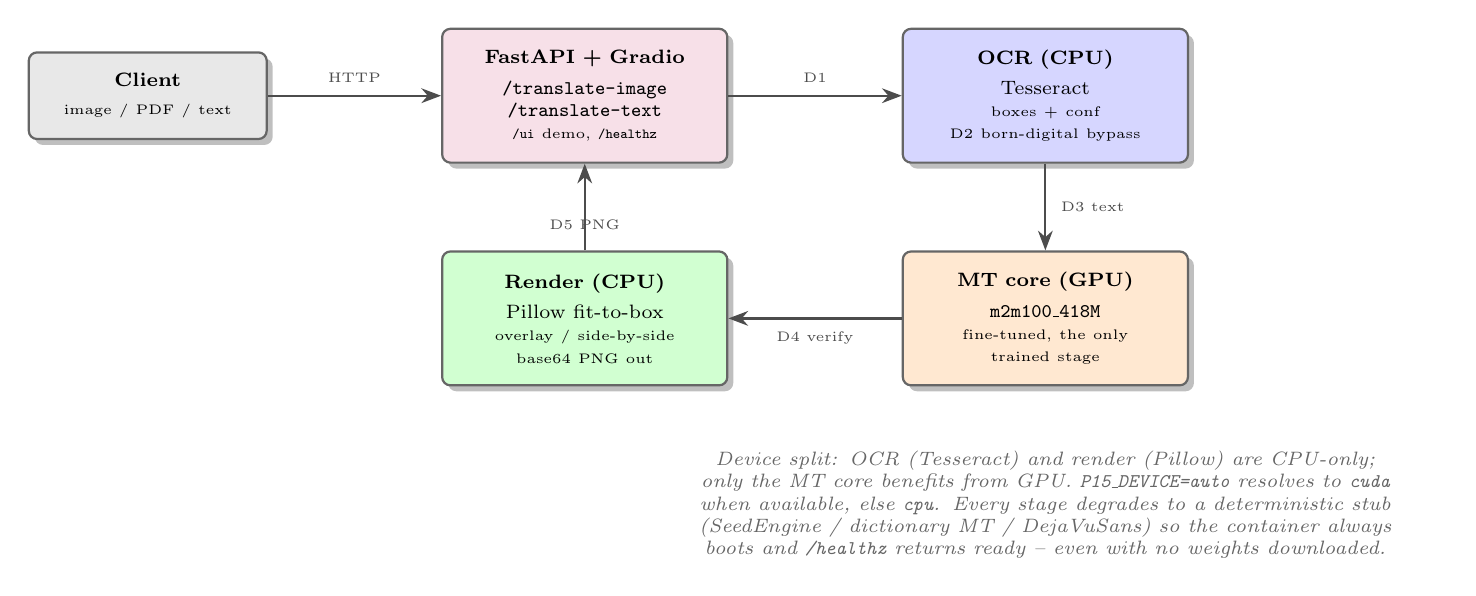
\begin{tikzpicture}[
  node distance=1.0cm and 2.2cm,
  box/.style={rectangle, draw=black!60, rounded corners=3pt, thick,
             text width=3.2cm, minimum height=1.7cm, align=center,
             inner sep=6pt, font=\scriptsize, drop shadow},
  ocrbox/.style={box, fill=blue!16},
  mtbox/.style={box, fill=orange!18},
  renderbox/.style={box, fill=green!18},
  apibox/.style={box, fill=purple!12},
  userbox/.style={box, fill=gray!18, text width=2.6cm, minimum height=1.1cm},
  note/.style={font=\scriptsize\itshape, align=center, text=black!60, text width=3.4cm},
  arrow/.style={-{Stealth[length=2.5mm]}, thick, color=black!70}
]

\node[userbox] (user) {%
  \textbf{Client}\\[2pt]
  {\tiny image / PDF / text}
};
\node[apibox, right=of user] (api) {%
  \textbf{FastAPI + Gradio}\\[3pt]
  \texttt{/translate-image}\\
  \texttt{/translate-text}\\
  {\tiny \texttt{/ui} demo, \texttt{/healthz}}
};
\node[ocrbox, right=of api] (ocr) {%
  \textbf{OCR (CPU)}\\[3pt]
  Tesseract\\
  {\tiny boxes + conf}\\
  {\tiny D2 born-digital bypass}
};
\node[mtbox, below=1.1cm of ocr] (mt) {%
  \textbf{MT core (GPU)}\\[3pt]
  \texttt{m2m100\_418M}\\
  {\tiny fine-tuned, the only}\\
  {\tiny trained stage}
};
\node[renderbox, below=1.1cm of api] (render) {%
  \textbf{Render (CPU)}\\[3pt]
  Pillow fit-to-box\\
  {\tiny overlay / side-by-side}\\
  {\tiny base64 PNG out}
};

\draw[arrow] (user) -- node[above=1pt, font=\tiny] {HTTP} (api);
\draw[arrow] (api) -- node[above=1pt, font=\tiny] {D1} (ocr);
\draw[arrow] (ocr) -- node[right=2pt, font=\tiny] {D3 text} (mt);
\draw[arrow] (mt) -- node[below=1pt, font=\tiny] {D4 verify} (render);
\draw[arrow] (render) -- node[below=1pt, font=\tiny] {D5 PNG} (api);

\node[note, below=0.7cm of mt, text width=10cm] {Device split: OCR (Tesseract) and render (Pillow) are CPU-only; only the MT core benefits from GPU. \texttt{P15\_DEVICE=auto} resolves to \texttt{cuda} when available, else \texttt{cpu}. Every stage degrades to a deterministic stub (SeedEngine / dictionary MT / DejaVuSans) so the container always boots and \texttt{/healthz} returns ready -- even with no weights downloaded.};

\end{tikzpicture}%
}
\caption{Deployment architecture. The agent (D1--D5) is the controller inside the FastAPI backend; the API is a thin transport layer that marshals bytes in and JSON/base64 out. The Gradio UI calls the same \texttt{imgtrans.agent} entrypoint, so the demo shows exactly what \texttt{/translate-image} returns.}
\label{fig:arch}
\end{figure}

\subsection{Endpoints}

\begin{table}[H]
\centering
\caption{FastAPI endpoints}
\small
\begin{tabularx}{\linewidth}{@{} l L @{}}
\toprule
\textbf{Endpoint} & \textbf{Behaviour} \\
\midrule
\texttt{GET /healthz} & Liveness/readiness; returns resolved runtime config (OCR engine + version, MT model + device, fonts, offline flag). \texttt{status="ok"} even in offline stub mode. \\
\texttt{POST /translate-text} & Text-in, text-out; \textbf{skips OCR + render} (the degenerate D1$\rightarrow$D4 path). Cheapest, GPU-MT-only. Returns translation + D4 verification (\texttt{round\_trip\_chrf}, \texttt{length\_ratio}, \texttt{status}). \\
\texttt{POST /translate-image} & Headline route: upload image/PDF $\rightarrow$ translated text \textbf{and} a base64 overlay PNG the same pixel size as input. Runs the full cascade through all five decision points. Gated on \texttt{python-multipart} (present in the Docker image). \\
\bottomrule
\end{tabularx}
\end{table}

A \texttt{/translate-image} response carries per-block \texttt{box}, \texttt{source}, \texttt{translation}, \texttt{ocr\_conf}, \texttt{font\_size}, \texttt{fit\_ok}, and \texttt{decision}; top-level \texttt{render\_mode} (\texttt{overlay} / \texttt{side\_by\_side} / \texttt{needs\_review}), a \texttt{layout} summary (\texttt{fit\_rate}, \texttt{mean\_shrink}, \texttt{overflow}), \texttt{verification}, the \texttt{overlay\_png\_base64}, and \texttt{needs\_review}. The error contract returns \texttt{200} even for \texttt{needs\_review:true} (a defensible non-destructive result, not an error), \texttt{400} for unsupported file types (D1), \texttt{413} for oversized uploads, \texttt{415} when the upload route is unavailable, and \texttt{422} for validation.

\subsection{GPU vs CPU and Latency}

The cascade has a clean device split that the deployment exploits: \textbf{OCR (Tesseract)} and \textbf{render (Pillow)} are CPU-only; \textbf{MT (m2m100)} is the only GPU-benefiting stage (fp16 on GPU is the throughput path, CPU fallback for the free-Space default). The latency budget for \texttt{/translate-image} is dominated, in order, by MT decode and OCR; render is sub-10ms per block. The born-digital PDF path (D2) bypasses OCR entirely -- the fastest image path with zero OCR error. \texttt{verify=true} (D4) doubles MT decode cost because of the round-trip back-translation, and can be disabled for throughput-critical batch jobs. All blocks above the D3 confidence gate are translated in a single batched MT call (the largest throughput win on multi-block pages).

\subsection{Docker}

The container ships the \textbf{Tesseract binary} (\texttt{tesseract-ocr} + \texttt{tesseract-ocr-fra} for the French source-side traineddata), \textbf{libGL} (required so PDF rasterization / imaging deps load on a slim base), Noto + DejaVu fonts, and \texttt{python-multipart} (enables the upload route). Configuration is 12-factor via environment variables, readable in \texttt{/healthz}: \texttt{P15\_SRC\_LANG}, \texttt{P15\_TGT\_LANG}, \texttt{P15\_DEVICE}, \texttt{P15\_MT\_MODEL}, \texttt{P15\_OFFLINE}, \texttt{P15\_OCR\_HIGH/LOW}, \texttt{P15\_VERIFY[\_TAU]}, \texttt{P15\_FIT\_MIN\_FONT}, \texttt{P15\_MAX\_UPLOAD\_MB}, \texttt{HF\_HOME}. \texttt{P15\_MT\_MODEL} must never be set to a non-commercial id in production.

% ============================================================
\section{Agentic AI Component}
% ============================================================

\subsection{What the Agent Is}

The \texttt{imgtrans} agent is a \textbf{deterministic finite-state machine (FSM)} that wraps the OCR $\rightarrow$ MT $\rightarrow$ render cascade -- not an LLM agent and not a learned policy. It routes on the pipeline's \emph{own intermediate signals} (file type, embedded-text coverage, OCR confidence, round-trip back-translation, length ratio, render-fit feasibility) and always emits a defensible output. Three properties define it:

\begin{itemize}\setlength\itemsep{0.15em}
  \item \textbf{Deterministic}: same input + same \texttt{AgentConfig} $\rightarrow$ byte-identical output; no randomness, no network required. This is what makes the offline seed evaluation reproducible.
  \item \textbf{Fail-soft}: every decision point has a degrade branch. Low-confidence OCR is skipped, not mistranslated; a translation that will not fit becomes side-by-side, not spilled text; anything genuinely uncertain becomes \texttt{needs\_review}.
  \item \textbf{Self-checking without a reference}: D4 uses the model's own back-translation and length statistics, so it needs no gold translation at inference time and works on real user uploads.
\end{itemize}

An optional LLM ``brain'' (\texttt{anthropic}) is \textbf{OFF by default} and, when enabled, \textbf{strictly advisory} -- it may annotate a borderline decision but never rewrites a translation, never overrides a D1--D5 branch, and never moves a threshold. The FSM remains the sole authority on routing.

\subsection{The Five-Decision Pipeline}

\begin{figure}[H]
\centering
\resizebox{0.96\linewidth}{!}{%
\begin{tikzpicture}[
  node distance=0.30cm,
  step/.style={rectangle, draw=black!60, rounded corners=2pt, thick,
              text width=13.2cm, inner sep=5pt, minimum height=0.7cm,
              align=center, font=\footnotesize},
  ingest/.style={step, fill=gray!15},
  ocr/.style={step, fill=blue!15},
  trans/.style={step, fill=orange!15},
  verify/.style={step, fill=purple!15},
  render/.style={step, fill=green!15},
  arrow/.style={-{Stealth[length=2mm]}, thick}
]

\node[ingest] (d1) {\textbf{D1 -- INGEST / input router + page-quality gate}: image $\rightarrow$ OCR; pdf $\rightarrow$ D2; \texttt{.txt} $\rightarrow$ skip OCR, jump to D4; unsupported $\rightarrow$ \texttt{needs\_review}};
\node[ocr, below=of d1] (d2) {\textbf{D2 -- OCR / born-digital vs scanned (PDF)}: PyMuPDF coverage $\geq$ thr $\rightarrow$ \textbf{use text layer, BYPASS OCR} (zero OCR error); else rasterize $\rightarrow$ Tesseract};
\node[trans, below=of d2] (d3) {\textbf{D3 -- TRANSLATE / per-block OCR-confidence gate}: conf $\geq$ 75 $\rightarrow$ MT; 40--75 $\rightarrow$ re-OCR (gamma/upscale/invert); $<$40 or garbage $\rightarrow$ drop + \texttt{needs\_review}};
\node[verify, below=of d3] (d4) {\textbf{D4 -- VERIFY / round-trip + length ratio}: rt-chrF $\geq \tau$ AND ratio $\in [0.4,3.0]$ $\rightarrow$ accept; rt $< \tau$ $\rightarrow$ re-decode once $\rightarrow$ else \texttt{low\_confidence} (soft, forward ratio to D5)};
\node[render, below=of d4] (d5) {\textbf{D5 -- RENDER / fit-feasibility gate}: \texttt{fit\_ok} at $\geq$ min font $\rightarrow$ \textbf{OVERLAY}; too long $\rightarrow$ \textbf{SIDE\_BY\_SIDE}; fit fails / D3/D4-flagged $\rightarrow$ \textbf{needs\_review}};

\foreach \a/\b in {d1/d2, d2/d3, d3/d4, d4/d5}
  \draw[arrow] (\a) -- (\b);

\end{tikzpicture}%
}
\caption{The deterministic five-decision FSM. Each state records a \texttt{ToolTrace} entry (step, decision + branch taken, measured signal, threshold, backend tool, block id) so every run is auditable and explainable. The only back-edges are the bounded single-shot retries inside D3 (re-OCR) and D4 (re-decode), so the FSM always terminates.}
\label{fig:agent}
\end{figure}

\subsection{Decision Table}

\begin{table}[H]
\centering
\caption{The five decision points (thresholds are \texttt{AgentConfig} defaults)}
\scriptsize
\setlength{\tabcolsep}{3pt}
\begin{tabularx}{\linewidth}{@{} l l L l L @{}}
\toprule
\textbf{Point} & \textbf{State} & \textbf{Intermediate signal} & \textbf{Threshold} & \textbf{Accept / degrade / fail} \\
\midrule
\textbf{D1} & ingest & MIME + magic-bytes + ext; page-quality & \texttt{supported\_*\_exts}; \texttt{min\_page\_dpi} & image$\rightarrow$ocr / pdf$\rightarrow$D2 / text$\rightarrow$D4 / spec$\rightarrow$SeedEngine; unsupported $\rightarrow$ \texttt{needs\_review} \\
\textbf{D2} & ocr (PDF) & PyMuPDF \texttt{get\_text()} coverage ratio & \texttt{born\_digital\_text\_ratio} & coverage $\geq$ thr $\rightarrow$ text layer, BYPASS OCR; else rasterize $\rightarrow$ OCR \\
\textbf{D3} & translate-in & Tesseract block mean conf + char sanity & \texttt{ocr\_conf\_high}$\approx$75, \texttt{ocr\_conf\_low}$\approx$40 & conf $\geq$ high $\rightarrow$ MT; low--high $\rightarrow$ re-OCR; $<$low / empty $\rightarrow$ drop + \texttt{needs\_review} \\
\textbf{D4} & verify & round-trip chrF; target/source length ratio & \texttt{roundtrip\_tau}$\approx$0.45; \texttt{[0.4, 3.0]} & rt$\geq\tau$ \& ratio in band $\rightarrow$ accept; rt$<\tau$ $\rightarrow$ re-decode once, else \texttt{low\_confidence}; out-of-band $\rightarrow$ forward to D5 \\
\textbf{D5} & render & \texttt{fit\_ok} from \texttt{fit\_box} + D4 ratio & \texttt{font\_size\_min}, \texttt{overlay\_fit\_rate\_min} & fits $\rightarrow$ OVERLAY; too long $\rightarrow$ SIDE\_BY\_SIDE; fit fails / flagged $\rightarrow$ \texttt{needs\_review} \\
\bottomrule
\end{tabularx}
\end{table}

\subsection{Value-Add: Why This Beats ``OCR $\rightarrow$ Translate $\rightarrow$ Print the String''}

A naive script reads text, translates it, and dumps the string. The agent adds the two things that separate a real camera-translate product from that script: (1) a \textbf{layout-preserving overlay with auto font-fit} -- translations drawn back where the source text was, with shrink-to-fit, wrapping, script-aware fonts, and erase-all-then-draw ordering; and (2) \textbf{confidence + verification gates on the model's own intermediate outputs} -- D3 so garbled text is never translated, D4 so MT hallucination/truncation is caught without any reference, and D5 so the system degrades \texttt{overlay $\rightarrow$ side\_by\_side $\rightarrow$ needs\_review} instead of overflowing boxes. Bonus: D2's born-digital bypass eliminates OCR error entirely on the common digital-PDF case.

\subsection{Example Interaction Traces}

\begin{lstlisting}
# Example 1 -- Clean English page -> OVERLAY
Input: notice_en.png  (a short, high-contrast English notice)
  D1 ingest : input_kind=image -> OCR path (raster; D2 no-op)
  D2 (n/a)  : raster image, no PDF text-layer probe
  D3 ocr    : block conf=91.3 >= 75 -> accept, send to MT
  D4 verify : round_trip_chrf=83.7, length_ratio=1.18 -> accept
  D5 render : fit_ok=true at font_size=28 -> OVERLAY (erase + re-render in box)
Output: render_mode=overlay, needs_review=false,
        layout={fit_rate:1.0, mean_shrink:1.0, overflow:0},
        overlay_png_base64="iVBORw0KGgo..." (same size as input)

# Example 2 -- Long French translation that overflows -> SIDE_BY_SIDE
Input: dense English paragraph (en->fr expands the text)
  D1 ingest : input_kind=image -> OCR path
  D3 ocr    : block conf=88 >= 75 -> accept
  D4 verify : length_ratio=2.6 (in band) but long -> forward ratio to D5
  D5 render : fit_ok=false at font_size_min (translation too long for box)
              -> SIDE_BY_SIDE (original untouched + translated caption panel)
Output: render_mode=side_by_side, needs_review=false
        (the expected en->fr / CJK->EN expansion case, not a bug)

# Example 3 -- Unreadable smudged block -> needs_review
  D3 ocr    : block conf=31 < ocr_conf_low(40) -> DROP block,
              skipped_blocks=[{reason:"low_ocr_conf"}] (never translate garbage)
  D5 render : block was D3-flagged -> needs_review (boxes + raw text, no destructive render)
Output: needs_review=true  (honest "please check" instead of a confident wrong overlay)
\end{lstlisting}

% ============================================================
\section{Continual Learning \& Monitoring}
% ============================================================

P15 is a cascade in which \textbf{only the MT stage is trained}, so continual learning means ``keep the MT checkpoint good and keep the cascade honest,'' not ``retrain a monolith.'' There is exactly \textbf{one model to retrain} but \textbf{three quality surfaces to monitor} (OCR, MT, layout) plus the agent's own routing decisions.

\subsection{Monitoring Strategy}

Every production request appends exactly one metrics-only row to a rolling JSONL job log (\texttt{runs/serve/jobs-YYYYMMDD.jsonl}), emitted by the agent's terminal state regardless of outcome (so logs are complete by construction). \textbf{The raw image and recognized text are NOT written to the job log by default} -- it holds metrics and routing decisions only. \texttt{monitoring/drift\_report.py} aggregates a window vs a frozen promotion-time baseline:

\begin{table}[H]
\centering
\caption{Monitoring surfaces and the agent signal each is fed by}
\small
\begin{tabularx}{\linewidth}{@{} l L l @{}}
\toprule
\textbf{Surface} & \textbf{Headline metric(s)} & \textbf{Signal (decision)} \\
\midrule
Routing health & needs-review / side-by-side / overlay rate & D1 / D5 final route \\
OCR quality & mean conf, low-conf-block rate, born-digital bypass rate & D3 conf; D2 router \\
Translation quality & round-trip chrF distribution, length-ratio dist., low-conf rate & D4 \\
Layout fidelity & fit-rate, mean shrink, overflow rate & D5 \texttt{fit\_box} \\
Latency / cost & p50/p95 total + per-stage (OCR / MT / render) & timing wrappers \\
\bottomrule
\end{tabularx}
\end{table}

Drift is flagged by \textbf{threshold drift} on headline scalars and \textbf{distribution drift} (PSI $>$ 0.2) on the length-ratio, round-trip-chrF, and OCR-confidence distributions. Crucially, \textbf{OCR drift and MT drift are attributed separately}: OCR is pretrained and not retrained by us, so OCR-confidence drift triggers an alert + investigation, never an MT retrain. The \textbf{born-digital-bypass slice} has zero OCR error by construction, so MT-quality drift measured there is a clean, OCR-free signal.

\subsection{Feedback and Continual Learning}

Feedback capture concentrates on the \texttt{side\_by\_side} and \texttt{needs\_review} pages -- exactly the failure tail most informative for retraining. A reviewer in the Gradio review tab supplies an optional corrected source / corrected target and a \texttt{human\_verdict} (\texttt{ocr\_wrong} / \texttt{mt\_wrong} / \texttt{both\_wrong} / \texttt{acceptable}) which routes the correction to the right stage: \texttt{mt\_wrong} becomes a high-value parallel pair; \texttt{ocr\_wrong} becomes an \emph{OCR-robustness} pair (corrupted source $\rightarrow$ gold target) so the MT core learns to translate \emph{through} that OCR noise. Corrections pass through \texttt{curate.py} (PII scrub + consent check, de-duplication, sanity filters, reviewer agreement) before entering a versioned, registered training mixture.

The retrain target is \textbf{always and only} \texttt{m2m100\_418M}, fine-tuned with the same \texttt{Seq2SeqTrainer} harness. A new checkpoint is promoted \textbf{only if} a champion--challenger gate passes: end-to-end image-translation chrF improves, clean-source MT chrF/BLEU does not regress, the feedback regression set stays \texttt{acceptable}, and projected needs-review rate does not rise. Promotion bumps the \texttt{model\_version} string and resets the drift baseline. Retraining is trigger-driven (calendar floor 1--3 months, feedback volume, MT-attributable quality/length-ratio drift on the bypass slice, needs-review rise, base-dependency bump) but always gated. The non-commercial NLLB/Surya options are hard-blocked from any promoted checkpoint.

% ============================================================
\section{Data Privacy \& Model Robustness}
% ============================================================

\subsection{Privacy}

Document images are an unusually sensitive input class -- IDs, passports, medical/legal/financial records -- and the raw image, the OCR'd text, and the rendered overlay can each leak the same PII. Privacy is therefore a first-class design constraint:

\begin{itemize}\setlength\itemsep{0.15em}
  \item \textbf{Local / on-device by default}: every shipped stage (Tesseract OCR, PyMuPDF router, local m2m100 weights, Pillow render) runs with \textbf{no network egress at inference time}. The only network access is at setup time (model/font/corpus download). A document is processed without leaving the machine.
  \item \textbf{No raw-image retention by default}: \texttt{/translate-image} processes the upload in memory, returns text + base64 overlay in the response, and does not persist the image, OCR text, or output. Any debug retention is opt-in and off by default.
  \item \textbf{The LLM brain is OFF by default}: the FSM needs no LLM; when off (the default), no document text or image is sent to any external API.
  \item \textbf{Minimisation}: block-level processing lets an operator translate only selected blocks; D3 \emph{drops} low-confidence blocks (never stores them); whiteout erase can be used to suppress a sensitive region.
\end{itemize}

\subsection{Robustness}

The input is uncontrolled pixels, and the synthetic generator's degradation suite (rotation, blur, noise, brightness/contrast jitter, JPEG recompression, plus a CLEAN-mode upper bound) means robustness is \emph{measured}, not assumed. Each realistic degradation has a recovery attempt and a graceful-fallback gate:

\begin{table}[H]
\centering
\caption{Robustness ladder: degradation $\rightarrow$ recovery $\rightarrow$ gate}
\small
\begin{tabularx}{\linewidth}{@{} L L L @{}}
\toprule
\textbf{Degradation} & \textbf{Recovery attempt} & \textbf{Gate / graceful fallback} \\
\midrule
Blur / skew / low DPI / noise & D3 retry: gamma / upscale / invert + re-score & conf $<$ LOW $\rightarrow$ drop block, \texttt{needs\_review} \\
Multi-column / complex layout & block/paragraph boxes; per-block render; erase-all-then-draw & no-overlap metric; side-by-side on bleed \\
Mixed scripts / RTL / CJK & target-aware Noto routing; per-char wrap; bidi shaping & DejaVu $\rightarrow$ \texttt{load\_default} glyph fallback (no crash) \\
OCR error $\rightarrow$ MT & D2 born-digital bypass; D3 pre-MT gate & D4 round-trip + length ratio $\rightarrow$ \texttt{low\_confidence} \\
Translation expansion & fit-to-box binary search (shrink-to-fit) & D5: overlay $\rightarrow$ side-by-side $\rightarrow$ \texttt{needs\_review} \\
Adversarial / garbled input & D1 magic-byte routing; D3 alpha/length sanity & unsupported / unreadable $\rightarrow$ \texttt{needs\_review} \\
Missing components (offline) & capability probes auto-select stubs & deterministic stub OCR / dict MT / DejaVu \\
\bottomrule
\end{tabularx}
\end{table}

The defining cascade risk -- OCR error propagating into MT -- is met by \textbf{three independent firewalls}: eliminate it where possible (D2 born-digital bypass = zero OCR error), stop bad text before MT (D3 confidence gate), and catch drift after MT (D4 round-trip + length ratio). The cross-cutting principle: \textbf{for a sensitive, hard-to-read document, the system prefers an honest \texttt{needs\_review} over a confident wrong answer.}

% ============================================================
\section{Project Management}
% ============================================================

This project was completed \textit{individually}. ``Division of work'' is organised by workstream so dependencies and reuse are explicit. The plan spans eight weeks of part-time effort across nine milestones; weeks overlap where a milestone is unblocked by an earlier deliverable.

\begin{table}[H]
\centering
\caption{Project timeline (eight-week plan, nine milestones)}
\small
\begin{tabularx}{\linewidth}{@{} l l L @{}}
\toprule
\textbf{Milestone} & \textbf{Week(s)} & \textbf{Key deliverable / exit criterion} \\
\midrule
M0 Research \& scaffold & 1 & Verify every HF id + license; flag non-commercial; offline smoke runs on stdlib + Pillow \\
M1 Synthetic generator & 1--2 & \texttt{synth\_render.py} hash-stable quadruples; committed fixtures (critical path) \\
M2 MT fine-tune core & 2--3 & m2m100 beats identity / dictionary / zero-shot on held-out opus-100 \\
M3 OCR integration & 3--4 & Tesseract \texttt{image\_to\_data} + PyMuPDF D2 router; SeedEngine; CER/WER \\
M4 Overlay render engine & 4--5 & \texttt{imaging/render.py} fit-to-box; verified Pillow case reproduces; fit-rate live \\
M5 Agentic FSM & 5--6 & D1--D5 route all three outcomes; runs fully offline \\
M6 End-to-end eval & 6 & All four metric families; clean-vs-degraded OCR-cost gap quantified \\
M7 Deploy & 7 & FastAPI + Gradio \texttt{/ui} + Docker; image upload $\rightarrow$ overlay PNG \\
M8 Hardening \& docs & 8 & Robustness pass; ethics/privacy; monitoring/grading/autopilot; final report \\
\bottomrule
\end{tabularx}
\end{table}

\textbf{Critical path}: M1 (generator) $\rightarrow$ M2 (MT) / M3 (OCR) $\rightarrow$ M4 (render) $\rightarrow$ M5 (agent) $\rightarrow$ M6 (eval). The generator is the most upstream dependency (it produces the gold that scores OCR, MT, end-to-end, and layout); M4$\rightarrow$M5 is the headline value-add, protected over deploy polish. \textbf{Reuse}: OCR plumbing + layout from \emph{P07 dococr}; the MT translator + chrF/BLEU metrics + config/logging/registry/autoreport/monitoring/grading/autopilot templates from \emph{P13 s2st / P14 doctrans}. \textbf{New for P15}: the \texttt{imaging/render.py} fit-to-box engine, the \texttt{synth\_render.py} generator, the SeedEngine offline OCR, and the five-decision agent.

% ============================================================
\section{Ethics \& Responsible AI}
% ============================================================

\subsection{The Tool Assists, It Does Not Decide}

The single most important ethical stance is that the system \textbf{never asserts certainty} about its own output. Every translated page is the product of three lossy stages (OCR, MT, render) stacked in series, and errors propagate forward -- a single OCR character error becomes a wrong word into MT, which becomes a confidently-rendered wrong translation. Because the output \emph{looks} like a finished typeset document, it carries unearned authority. The agentic design exists to counteract that: the system surfaces its own uncertainty (per-block confidence, the chosen output mode, the \texttt{needs\_review} flag) rather than hiding it behind a clean render.

\subsection{Who Benefits, Who Could Be Harmed}

\textbf{Benefits} accrue to newcomers, migrants, and travelers who can read a letter, form, or sign without a human translator; layout preservation matters for comprehension (a translated form whose fields stay in place is usable); born-digital PDFs are translated losslessly; and multilingual coverage comes from one checkpoint. \textbf{Harms} arise if a mistranslation in a high-stakes document (passport, prescription, contract, court filing) is relied upon. P15 must never substitute for a certified human translator in legal or medical contexts; the design enforces ``assist, do not assert'' through concrete gates (D3 never translates garbage; D4 catches hallucination/truncation without a reference; D5 degrades instead of faking success), and \textbf{a competent human must review the output before it is relied upon}.

\subsection{Bias}

Bias enters in two independent places and compounds. \textbf{MT bias}: translating into gendered languages (e.g. French) forces gender assignments the source left unspecified; non-standard dialects and registers translate less well; m2m100 quality is far from uniform across its $\sim$100 languages. \textbf{OCR bias}: Tesseract is strongest on Latin print and weaker on complex scripts (Arabic, Devanagari, Thai), CJK, handwriting, and decorative type, so a less-supported script enters MT already more corrupted. The commitment is to \textbf{measure and disclose}, not claim to have removed, bias: metrics are reported \emph{per language pair and per condition}, never a single headline number that hides disparity, and the honest non-saturated floor is reported on real opus-100 pairs (not the saturated seed).

\subsection{Licensing as an Ethical Choice}

Choosing a fully-permissive default is itself an ethical choice: it keeps the tool freely usable and avoids quietly violating a non-commercial term. The higher-quality but non-commercial \texttt{nllb-200-distilled-600M} (CC-BY-NC-4.0) and Surya OCR (CC-BY-NC-SA-4.0) are \textbf{flagged and never shipped}; each \texttt{opus-100} pair's license must be verified before commercial use.

\paragraph{One-line ethic.} \emph{Translate what it can read, flag what it cannot, never assert certainty, keep the original for a human -- and treat every document image as if it contains someone's private, high-stakes information, because it often does.}

% ============================================================
\section{Conclusion \& Future Work}
% ============================================================

\subsection{Summary}

\begin{itemize}\setlength\itemsep{0.15em}
  \item A complete, license-clean, production-grade in-image translation pipeline: a cascade OCR $\rightarrow$ MT $\rightarrow$ layout-preserving render, with \texttt{m2m100\_418M} (MIT) the single trained stage.
  \item A deterministic five-decision agent (D1--D5) with a self-checking degradation ladder (\texttt{overlay} $\rightarrow$ \texttt{side\_by\_side} $\rightarrow$ \texttt{needs\_review}) that produces a defensible output on every input.
  \item A reproducible synthetic generator that constructs the \texttt{(image, gold\_src, gold\_tgt, boxes)} quadruples no public benchmark provides, enabling four exact metric families.
  \item Verified offline seed floor: dictionary chrF \textbf{79.9} vs identity \textbf{22.4}, OCR CER \textbf{0.0}, end-to-end chrF \textbf{76.4}, fit-rate \textbf{1.0}, grade \textbf{0.97}, all 5 decisions fire, 22 tests pass -- proving the cascade is wired and every metric computes. The honest quality story (fine-tuned m2m100 dominating on held-out opus-100) lives on the real Colab H100 run.
  \item Deployable as REST API + Gradio UI + Docker + a one-button Colab H100 autopilot; PII-aware, local-by-default privacy posture; every shipped component MIT/Apache-2.0/OFL/CC0.
\end{itemize}

\subsection{Future Work}

\begin{enumerate}\setlength\itemsep{0.15em}
  \item \textbf{A real held-out benchmark}: if a license-clean, \texttt{hub\_repo\_details}-verified in-image translation set is located, wire it in as a held-out test split.
  \item \textbf{Quality upgrades (H100 tier)}: swap MT to \texttt{mbart-large-50-many-to-many-mmt} (MIT) and the OCR recognizer to \texttt{trocr-large-printed} / \texttt{GOT-OCR-2.0-hf} for tough photographs -- all permissive, drop-in behind the same interfaces.
  \item \textbf{Better erase}: improve the whiteout on textured / multi-color backgrounds (simple-inpaint smear + blur), short of a neural inpainter.
  \item \textbf{RTL shaping}: ship \texttt{python-bidi} + \texttt{arabic-reshaper} for correct Arabic/Hebrew shaping rather than best-effort logical-order drawing.
  \item \textbf{Real-time monitoring}: a drift dashboard reading the JSONL job logs, with per-language and per-condition alerting and an automated champion--challenger retrain.
\end{enumerate}

% ============================================================
\newpage
\begin{thebibliography}{9}

\bibitem{m2m100} Fan, A., et al. (2021). Beyond English-Centric Multilingual Machine Translation (\textit{m2m100}). \textit{JMLR}. Model: \url{https://huggingface.co/facebook/m2m100_418M}

\bibitem{tesseract} Smith, R. (2007). An Overview of the Tesseract OCR Engine. \textit{ICDAR 2007}. \url{https://github.com/tesseract-ocr/tesseract}

\bibitem{pymupdf} Artifex / PyMuPDF. \textit{PyMuPDF (fitz) -- Python bindings for MuPDF}. \url{https://pymupdf.readthedocs.io/}

\bibitem{pillow} Clark, A. and contributors. \textit{Pillow -- the friendly PIL fork}. \url{https://python-pillow.org/}

\bibitem{opus100} Zhang, B., Williams, P., Titov, I., \& Sennrich, R. (2020). Improving Massively Multilingual Neural Machine Translation and Zero-Shot Translation (\textit{OPUS-100}). \textit{ACL 2020}.

\bibitem{chrf} Popovi\'c, M. (2015). chrF: Character n-gram F-score for Automatic MT Evaluation. \textit{WMT 2015}; \texttt{sacrebleu}: Post, M. (2018). \textit{WMT 2018}.

\bibitem{huggingface} Wolf, T., et al. (2020). Transformers: State-of-the-Art Natural Language Processing. \textit{EMNLP 2020}.

\bibitem{fastapi} Ram\'irez, S. (2018). FastAPI. \url{https://fastapi.tiangolo.com/}

\bibitem{gradio} Abid, A., et al. (2019). Gradio. \url{https://www.gradio.app/}

\bibitem{noto} Google. \textit{Noto Fonts} (SIL OFL 1.1). \url{https://fonts.google.com/noto}

\end{thebibliography}

\end{document}
